\subsection{CUDA Parellized Algorithms}
\subsubsection{Time Domain Convolution}
\paragraph{Algorithm Selection} \hspace{0pt} \\
\indent \par For time domain convolution, I tried four different algorithms with different optimization techniques which I labelled as: Atomic, Atomic Shared, Naive, and Excessive.

\begin{minted}[breaklines, breakanywhere]{cuda}
#define tile 512

__global__ void timeDomainConvolutionAtomic(float *ibuf, float *fbuf, float *obuf, long long iFrames, long long fFrames){
	int threadID = blockIdx.x * blockDim.x + threadIdx.x;
	float h;
	if(threadID < fFrames){
		h = fbuf[threadID];
		for(int i = 0; i < iFrames; i++){
			atomicAdd(obuf + threadID  + i , ibuf[i] * h);
		}
	}
	
}

__global__ void timeDomainConvolutionAtomicShared(float *ibuf, float *fbuf, float *obuf, long long iFrames, long long fFrames){
	__shared__ float x[tile];
	int threadID = blockIdx.x * blockDim.x + threadIdx.x;
	int numLoops = (iFrames + tile - 1) / tile;
	float h = 0.0f;
	if(threadID < fFrames){
		h = fbuf[threadID];
	}
	for(int n = 0; n < numLoops; n++){
		if(n * tile + threadIdx.x < iFrames){
			x[threadIdx.x] = ibuf[n * tile + threadIdx.x];
		}
		__syncthreads();
		for(int i = 0; i < tile; i++){
			if(n * tile + i < iFrames){
				atomicAdd(obuf + threadID + (n * tile) + i , x[i] * h);
			}
		}
		__syncthreads();
	}

}

__global__ void timeDomainConvolutionNaive(float *ibuf, float *fbuf, float *obuf, long long iframes, long long fFrames){
	int threadID = blockIdx.x * blockDim.x + threadIdx.x;
	if(threadID < iframes + fFrames - 1){
		int i_size = iframes;
		float value = 0;
		for(int k = 0; k < fFrames; k++){
			if(threadID - k >= 0 && threadID - k <= i_size){
				value += ibuf[threadID - k] * fbuf[k];
			}
		}
		obuf[threadID] = value;
	}
}

__global__ void timeDomainConvolutionExcessive(float *ibuf, float *fbuf, float *obuf, long long iFrames, int chunkNo){
	__shared__ float x[tile];
	__shared__ float h;
	
	if(chunkNo * tile + threadIdx.x < iFrames){
		x[threadIdx.x] = ibuf[chunkNo * tile + threadIdx.x];
	}
	h = fbuf[blockIdx.x];
	__syncthreads();
	if(chunkNo * tile + threadIdx.x < iFrames){
		atomicAdd(obuf + blockIdx.x + chunkNo * tile + threadIdx.x, x[threadIdx.x] * h);
	}
}
...
    /*ATOMIC*/
	numBlocks = (smallerFrames + numThreads - 1) / numThreads;
	timeDomainConvolutionAtomic<<< numBlocks, numThreads >>> (d_biggerBuf, d_smallerBuf, d_atomic, biggerFrames, smallerFrames);
	
	/*ATOMIC SHARED*/
	numBlocks = (smallerFrames + tile - 1) / tile;
	timeDomainConvolutionAtomicShared<<<numBlocks, tile >>>(d_biggerBuf, d_smallerBuf, d_atomic_shared, biggerFrames, smallerFrames);

	/*NAIVE*/
	numBlocks = (oFrames + numThreads - 1) / numThreads;
	timeDomainConvolutionPlain<<<numBlocks, numThreads >>>(d_biggerBuf, d_smallerBuf, d_naive, biggerFrames, smallerFrames);

	/*EXCESSIVE*/
	int numChunks = (biggerFrames + tile - 1) / tile;
	cudaStream_t streams[numChunks];
	for(int i = 0; i < numChunks; i++){
		checkCudaErrors(cudaStreamCreate(&streams[i]));
		timeDomainConvolutionExcessive<<<smallerFrames, tile, 0, streams[i]>>>(d_biggerBuf, d_smallerBuf, d_excessive, biggerFrames, i);
	}
...
\end{minted}

I lightly tested all of these and determined the accuracy of all of these algorithms based off a CPU-generated reference. In this test, K = 480,000 and N = 2,304,000. All trials were done on different \glspl{gpu}, but each trial was done on the same \gls{gpu}. 



For this experiment, the lower the time and smaller the accuracy, the better. So the naive algorithm is the winner. This is most likely do to the fact that the naive algorithm is the only gather decomposition algorithm. 
%\newpage
\begin{center}
Accuracy and Performance of Time Domain Convolution
\begin{tabular}{c c c c c}
 & Atomic & Atomic Shared & Naive & Excessive\\ 
 \textbf{TRIAL 1 }& & & \\
 Time (ms) & 61,269.718750 & 55,455.371094 &  19,140.958984 & 85,790.375000 \\  
 Accuracy & 3.981590E-05 & 5.722046E-05 & 2.622604E-06 & 1.606941E-04 \\
 \textbf{TRIAL 2} & & & \\
 Time (ms) & 37,341.425781  & 39,479.070312 & 7,031.311035 & 891,233.000000  \\
 Accuracy & 5.817413E-05 & 3.738447E+00 & 2.622604E-06 & 1.604557E-04 \\
 \textbf{TRIAL 3} & & & \\
 Time (ms) & 44,167.503906 & 46,413.277344 & 6,294.338867 & 747,803.625000 \\
 Accuracy & 4.386902E-05 & 3.738448E+00 & 2.622604E-06 & 1.602173E-04 \\
 \textbf{TRIAL 4} & & & \\
 Time (ms) & 53,322.039062 & 59,273.648438 & 11,514.409180 & 3,607,842.000000\\
 Accuracy & 5.626678E-05 & 3.886223E-05 & 2.622604E-06 & 1.604557E-04 \\
 \textbf{TRIAL 5} & & & \\
 Time (ms) & 62,557.585938 & 55,986.953125 & 19,912.279297 & 456,349.562500 \\
 Accuracy & 5.173683E-05 & 3.738460E+00 & 2.622604E-06 & 1.609325E-04 \\
 
\end{tabular}
\end{center}
\paragraph{Parallelized Peak Scaling} \hspace{0pt} \\
\indent For the finding the peak of the input and output, I used a library called Thrust. In Thrust, there is an API to find the extrema of an array \citep{thrust}.

\begin{minted}[breaklines, breakanywhere]{cuda}
__host__ __device__ thrust::pair<ForwardIterator,ForwardIterator> thrust::minmax_element(const thrust::detail::execution_policy_base< DerivedPolicy > &exec, ForwardIterator first, ForwardIterator last);
\end{minted}

This \gls{api} is called \verb|minmax_element()|. The first argument is either \verb|thrust::host| or \verb|thrust::device| depending on if the data is on the host or the device. These are special execution policies within Thrust. The second argument and third arguments are pointer wrappers to the first and last (exclusively last) element. The function returns a structure that contains two of these pointer wrappers, one for the minimum element and one for the maximum element in this array. Essentially, it takes in two addresses, scans all the values inbetween them, and returns two addresses. This is how I used it:
\begin{minted}[breaklines, breakanywhere]{cuda}

/*Functions to find extrema*/
float DExtrema(float *pointer, long long size){
	/*Convert raw float pointer into a thrust device pointer*/
	thrust::device_ptr<float> thrust_d_signal(pointer);
	
	thrust::pair < thrust::device_ptr<float>, thrust::device_ptr<float> >pair = thrust::minmax_element(thrust::device, thrust_d_signal, thrust_d_signal + size);
	float *d_min, *d_max;
	float min = 0, max = 0;
	
	d_min = pair.first.get();
	d_max = pair.second.get();
	
	checkCudaErrors(cudaMemcpy(&min, d_min, sizeof(float), cudaMemcpyDefault));
	checkCudaErrors(cudaMemcpy(&max, d_max, sizeof(float), cudaMemcpyDefault));

	return std::abs(min) > max ? std::abs(min) : max;
}


\end{minted}

I also have a kernel to scale all real numbers:

\begin{minted}[breaklines, breakanywhere]{cuda}

__global__ void RealFloatScale(float *a, long long size, float scale) {
	int numThreads = blockDim.x * gridDim.x;
	int threadID = blockIdx.x * blockDim.x + threadIdx.x;
	for (; threadID < size; threadID += numThreads) {
		a[threadID] *= scale;
	}
}
\end{minted}

\paragraph{Abridged Time Domain Convolution Code} \hspace{0pt} \\
\indent Put together, this is my abridged time domain convolution code, where \verb|**d_ibuf| is the input allocated on the device, and \verb|**d_fbuf| is the filter allocated on the device.
\begin{minted}[breaklines, breakanywhere]{cuda}
__global__ void timeDomainConvolutionNaive(float *ibuf, float *fbuf, float *obuf, long long iframes, long long fframes){
	int threadID = blockIdx.x * blockDim.x + threadIdx.x;
	if(threadID < iframes + fframes - 1){
		float value = 0;
		for(int k = 0; k < fframes; k++){
			if(threadID - k >= 0 && threadID - k <= fframes){
				value += ibuf[threadID - k] * fbuf[k];
			}
		}
		obuf[threadID] = value;
	}
}
float *TDconvolution(float ** d_ibuf, float ** d_fbuf, long long iFrames, long long oFrames){
    float *d_obuf, *obuf;
    long long fFrames = oFrames - iFrames + 1;

    /*Allocate device and host memory for the output*/
    checkCudaErrors(cudaMalloc(&d_obuf, oFrames * sizeof(float)));
    checkCudaErrors(cudaMallocHost((void**)&obuf, oFrames * sizeof(float)));

    /*Find peak of input*/
    float minmax = DExtrema(*d_ibuf, old_size);

    /*Launch the convolution  kernel*/
    int numThreads = 512;
    int numBlocks = (oFrames + numThreads - 1) /    numThreads;
    timeDomainConvolutionNaive<<<numBlocks, numThreads>>> (*d_ibuf, *d_fbuf, d_obuf, iFrames, fFrames);
    checkCudaErrors(cudaDeviceSynchronize());

    /*Find peak of output*/
    float minmax2 = DExtrema(d_obuf, oFrames);
    float scale = minmax/minmax2;

    /*Launch scaling kernel*/
    RealFloatScale <<< numBlocks, numThreads >>> (d_obuf, oFrames, scale);
    checkCudaErrors(cudaDeviceSynchronize());

    /* Copy device memory to host */
    checkCudaErrors(cudaMemcpy(obuf, d_obuf, oFrames * sizeof(float), cudaMemcpyDeviceToHost));

    checkCudaErrors(cudaFree(d_obuf));
    checkCudaErrors(cudaFree(*d_ibuf));
    checkCudaErrors(cudaFree(*d_fbuf));
    return obuf;
}
\end{minted}
\subsubsection{Frequency Domain Convolution}
\indent \par CUDA has an \gls{fft} library called cuFFT. The library was modeled after FFTW, and there is actually an interface to FFTW to allow people to easily port from FFTW to cuFFT. Just like in FFTW, there are \gls{fft} plans that need to be created, and there is an \gls{api} for R2C and C2R transforms to save time and memory capacity. The \glspl{api} look like this \citep{cufft}.

\begin{minted}[breaklines, breakanywhere]{cuda}
    cufftResult_t cufftCreate(cufftHandle* plan);
    cufftResult_t cufftPlan1d(cufftHandle* plan, int nx, cufftType type, int batch);
    cufftResult_t cufftExecR2C(cufftHandle plan, cufftReal *idata, cufftComplex *odata);
    cufftResult_t cufftExecC2R(cufftHandle plan, cufftComplex *idata, cufftReal *odata);
    cufftResult_t cufftDestroy(cufftHandle plan);
\end{minted}

These are incredibly similar to the FFTW plans. For the pointwise multiplication, there is a kernel with a modular function:

\begin{minted}[breaklines, breakanywhere]{cuda}
 __device__ __host__ inline Complex ComplexMul(Complex a, Complex b) {
	Complex c;
	c.x = a.x * b.x - a.y * b.y;
	c.y = a.x * b.y + a.y * b.x;
	return c;
}

__global__ void ComplexPointwiseMul(Complex *a, const Complex *b, int size) {
	const int numThreads = blockDim.x * gridDim.x;
	const int threadID = blockIdx.x * blockDim.x + threadIdx.x;
	for (int i = threadID; i < size; i += numThreads) {
		a[i] = ComplexMul(a[i], b[i]);
	}
}
\end{minted}

So the basic code looks like this: 

\begin{minted}[breaklines, breakanywhere]{cuda}
/*float **d_ibuf, float **d_fbuf, long long iFrames, long long fFrames, long long size are passed in*/
    
    /*Allocate memory for complex signal & filter*/

    /*Create FFT plans*/
    cufftHandle plan, outplan;
    CHECK_CUFFT_ERRORS(cufftPlan1d(&plan, size, CUFFT_R2C, 1));
    CHECK_CUFFT_ERRORS(cufftPlan1d(&outplan, size, CUFFT_C2R, 1));

    /*Transform Complex Signal*/
    CHECK_CUFFT_ERRORS(cufftExecR2C(plan, (cufftReal *) *d_ibuf, d_sig_complex));

    /*Transform Filter Signal*/
    CHECK_CUFFT_ERRORS(cufftExecR2C(plan, (cufftReal*) *d_fbuf, d_filter_complex));

    /*Convolution*/
    int blockSize = 256;
    int numBlocks = (size + blockSize - 1) / blockSize;
	
    ComplexPointwiseMul << < numBlocks, blockSize >> > (d_sig_complex, d_filter_complex, size / 2 + 1);

    /*IFFT*/
    CHECK_CUFFT_ERRORS(cufftExecC2R(outplan, d_sig_complex, *d_ibuf));
    
    /*Scale the output according to the input*/
    /*Copy to host*/
    /*Cleanup memory*/
\end{minted}
\paragraph{cuFFT Callback Routine} \hspace{0pt} \\
\indent There is a special \gls{api} in the cuFFT library that allows for functions to modify the data before and/or after a transform, and it is embedded within the transform. These are custom cuFFT callbacks. According to NVIDIA, larger input sizes can improve performance by 20\% \citep{cufft_callbacks}. Modifying the data before the transform is known as a load callback, and modifying the data after the transform is known as a store callback. cuFFT supports several different types of transforms, so there are a total of 8 different callback types. 

Convolution can utilize a load callback into the inverse, C2R. The load callback will modify complex data on a point-by-point basis before sending it to the C2R. This is function prototype for the load callback \citep{cufft}.

\begin{minted}[breaklines, breakanywhere]{cuda}
    typedef cufftComplex (*cufftCallbackLoadC)(void *dataIn, size_t offset, void *callerInfo, void *sharedPointer);
\end{minted}

A callback needs to be defined, and then a device pointer to the callback routine must be defined. The host then must copy this device pointer and pass it to cuFFT. The setup syntax looks like this:
\begin{minted}[breaklines, breakanywhere]{cuda}
    /*Declarations/Definitions*/
    __device__ __host__ inline Complex ComplexMul(Complex a, Complex b) {
    	Complex c;
    	c.x = a.x * b.x - a.y * b.y;
    	c.y = a.x * b.y + a.y * b.x;
    	return c;
    }
    __device__ cufftComplex cbComplexPointwiseMul(void *dataIn, size_t offset, void *cb_info, void *sharedmem) {
	    cufftComplex *filter = (cufftComplex*)cb_info;
	    return (cufftComplex) ComplexMul(((Complex *)dataIn)[offset], filter[offset]);
	}
	
    // Define the device pointer to the callback routine. 
    __device__ cufftCallbackLoadC myOwnCallbackPtr = cbComplexPointwiseMul;
\end{minted}

This means that I don't have to use the complex multiplication kernel explicitly. The convolution section of the code with the callback looks like this:

\begin{minted}[breaklines, breakanywhere]{cuda}
    /*float **d_ibuf, float **d_fbuf, long long iFrames, long long fFrames, long long size are passed in*/
    
    /*Allocate memory for complex signal & filter*/
    
    /*Create FFT plans*/
    cufftHandle plan, outplan;
    CHECK_CUFFT_ERRORS(cufftPlan1d(&plan, size, CUFFT_R2C, 1));
    CHECK_CUFFT_ERRORS(cufftPlan1d(&outplan, size, CUFFT_C2R, 1));
	
    /*Transform Signals*/
    CHECK_CUFFT_ERRORS(cufftExecR2C(plan, (cufftReal *)*d_ibuf, d_sig_complex));
    CHECK_CUFFT_ERRORS(cufftExecR2C(plan, (cufftReal*)*d_fbuf, d_filter_complex));
	
    /*Copy over the host copy of callback function*/
    cufftCallbackLoadC hostCopyOfCallbackPtr;
    checkCudaErrors(cudaMemcpyFromSymbol(&hostCopyOfCallbackPtr,myOwnCallbackPtr, sizeof(hostCopyOfCallbackPtr)));
	
    /*Associate the load callback with the plan*/
    CHECK_CUFFT_ERRORS(cufftXtSetCallback(outplan, (void **)&hostCopyOfCallbackPtr, CUFFT_CB_LD_COMPLEX, (void **)&d_filter_complex));

    /*Transform signal back, callback pointwise multiplies on the way in*/
    CHECK_CUFFT_ERRORS(cufftExecC2R(outplan, d_sig_complex, *d_ibuf));
	
    /*Scale the output according to the input*/
    /*Copy to host*/
    /*Cleanup memory*/
\end{minted}
\paragraph{In-Place Overlap-Add within one GPU} \hspace{0pt} \\
\indent Frequency domain convolution takes up extra memory to account for the complex arrays. cuFFT itself needs some spare scratch space called a workspace to be able to do the computations. Because of this, the input could be too big to fit on the \gls{gpu}. To account for that, the input can be divided into chunks and convolved chunk by chunk, as described earlier. To make sure that we don't run out of space, we can do in-place overlap-add. The algorithm is the same as detailed in the Sequential Frequency Domain section, but in-place adds more steps.

To find the block amount ($M + L$), I use a few \glspl{api}. Whatever the block size is, there will be four arrays of that size in bytes - two for complex and two for real. So the total amount of memory to allocate will approximately be \verb|blockSize * 16|. There's a couple memory \glspl{api} that I used to calculate the maximum size of the block that will fit on the device \citep{cufft}, \citep{cudaC}.

\begin{minted}[breaklines, breakanywhere]{cuda}
    cufftResult cufftEstimate1d(int nx, cufftType type, int batch, size_t *workSize);
    cudaResult_t cudaMemGetInfo(size_t *free, size_t *total);
\end{minted}

\verb|cufftEstimate1d()| fills workSize with the amount of space it should take to perform the transform. \verb|cudaMemGetInfo()| returns the amount of free and total global memory left on the device. To find the maximum size of the block that will fit on the device, I used a loop and overestimated the amount of bytes to be 18x the block size instead of 16:

\begin{minted}[breaklines, breakanywhere]{cuda}
int myExp = ceil(log2((float)(iFrames + M)));
size_t blockSize = pow(2, myExp);
int L = iFrames, blockNum = 0;
size_t workspace;
CHECK_CUFFT_ERRORS(cufftEstimate1d(blockSize, CUFFT_R2C, 2, &workspace));
while(getFreeSize() < workspace + blockSize * 18L){
	myExp--;
	blockSize = pow(2, myExp);
	blockNum++;
	CHECK_CUFFT_ERRORS(cufftEstimate1d(blockSize, CUFFT_R2C, 2, &workspace));
}
\end{minted}

This is what the in-place algorithm looks like, along with matching code.

\def\excerpt{\thispagestyle{empty} \paragraph{In-Place Overlap-Add Algorithm} \hspace{0pt} \\}
\includepdf[pages=5, scale=0.95,
pagecommand={\excerpt}]{Algorithms.pdf}

\begin{minted}[breaklines, breakanywhere]{cuda}
/*Memory has been allocated, number of blocks has been determined*/
/*Callback function has been set and attached to outplan*/
/*Filter has already been transformed above*/
for(int blockNo = 0; blockNo <= blockNum; blockNo++){
	long long cpyAmount = L;
	if (blockNo == blockNum) {
		cpyAmount = iFrames % L;
	}
	checkCudaErrors(cudaMemcpy(d_padded_signal, &d_obuf[L * blockNo], cpyAmount * sizeof(float), cudaMemcpyDeviceToDevice));
	
	if (blockNo != 0) {
		checkCudaErrors(cudaMemcpy(&d_obuf[L * blockNo], &d_padded_signal[L], M * sizeof(float), cudaMemcpyDeviceToDevice));
	}
	
	/*fillWithZeroes is a wrapper to a thrust API to fill with 0's. Params: (array, start, end)*/
	fillWithZeroes(&d_padded_signal, cpyAmount, blockSize);
	
	/*Transform signal*/
	CHECK_CUFFT_ERRORS(cufftExecR2C(plan, (cufftReal *)d_padded_signal, d_sig_complex));

	/*IFFT*/
	CHECK_CUFFT_ERRORS(cufftExecC2R(outplan, d_sig_complex, d_padded_signal));
	if (blockNo != 0) {
		PointwiseAdd << <numBlocks, numThreads >> > (d_padded_signal, &d_obuf[blockNo * L], M);
	}
	
	/*Initial case*/
	if (blockNo == 0) {
	    checkCudaErrors(cudaMemcpy(d_obuf, d_padded_signal, L * sizeof(float), cudaMemcpyDeviceToDevice));
	}
	/*Last case*/
	else if (blockNo == blockNum) {
		checkCudaErrors(cudaMemcpy(&d_obuf[blockNo * L + M], &d_padded_signal[M], cpyAmount * sizeof(float), cudaMemcpyDeviceToDevice));
	}
        /*Every other case*/
        else{
		checkCudaErrors(cudaMemcpy(&d_obuf[blockNo * L + M], &d_padded_signal[M], (L - M) * sizeof(float), cudaMemcpyDeviceToDevice));
	}
}
\end{minted}
\paragraph{Overlap-Add with multiple GPUs} \hspace{0pt} \\
\indent This same concept of overlap-add can be used on multiple \glspl{gpu} instead of just one. Several servers have multiple cards, and they can be accessed in CUDA code individually. This way, all asynchronous calls will run at the same time. This is used through \verb|cudaSetDevice(int devNum)|. 

The approach I used is to find out the largest block that can fit on each card and fill each one until there are no more input samples left to distribute. This would involve finding the amount of free space on the card and dividing by a the number of bytes I plan to allocate (plus more to be conservative and prevent allocation errors). Once the largest size that can fit on the device is discovered, subtract $K-1$ to find the amount of input samples that can be convolved on the device. This does not distribute the input evenly, and there is a potential that all the cards are not being used. I had an array called \verb|size_t inSizes[numDevices]| where I stored the block sizes for each device.

\begin{minted}[breaklines, breakanywhere]{cuda}
/*numDevs = number of devices
getFreeSize() returns the free amount in global memory on the device
size_t inSizes[] is an array to store the block size per device
d_ibufs is the input array
iFrames = input size
M = fFrames - 1
*/
size_t freeSizes[numDevs];
/*Find out amount of free memory on each device*/
for (int i = 0; i < numDevs; i++) {
    cudaSetDevice(i);
    freeSizes[i] = getFreeSize();
    /*most precise is input = freeSize()/16 - 16, but dividing by 32 to conservatively account for cuFFT space*/
    size_t freeSize = freeSizes[i] / 32;
    /*max number of elements that's a power of 2*/
    inSizes[i] = pow(2, floor(log2((double)freeSize)));
}
/*Allocate the block amount, stop if we've used all of the input*/
long long frames = 0;
for(int i = 0; i < numDevs; i++){
    cudaSetDevice(i);
    if(frames >= iFrames){
        inSizes[i] = 0;
        continue;
    }
    frames += inSizes[i] - M;
    checkCudaErrors(cudaMalloc(&d_ibufs[i], inSizes[i] * sizeof(float)));
    checkCudaErrors(cudaMalloc(&d_rbufs[i], inSizes[i] * sizeof(float)));
    checkCudaErrors(cudaMalloc(&d_Cbufs[i], (inSizes[i] + 2) * sizeof(cufftComplex)));
}
/*Copy memory to devices and pad with zeros. Do the 4 tasks in 4 different streams per device*/
int streamsPerDev = 4;
cudaStream_t stream[numDevs * streamsPerDev];
for(int i = 0; i < numDevs; i++){
    cudaSetDevice(i);
    checkCudaErrors(cudaStreamCreate(&stream[i * streamsPerDev]));
    checkCudaErrors(cudaStreamCreate(&stream[i * streamsPerDev + 1]));
    checkCudaErrors(cudaStreamCreate(&stream[i * streamsPerDev + 2]));
    checkCudaErrors(cudaStreamCreate(&stream[i * streamsPerDev + 3]));
    if (inSizes[i] == 0){
        continue;
    }
    long long amtRead = inSizes[i] - M;
    if (frames + amtRead > iFrames){
        amtRead = iFrames - frames;
    }
    checkCudaErrors(cudaMemcpyAsync(d_ibufs[i], ibuf + frames, amtRead * sizeof(float), cudaMemcpyHostToDevice, stream[i * streamsPerDev]));
    numBlocks = (inSizes[i] - amtRead + blockSize - 1 ) / blockSize;
    FillWithZeros<<<numBlocks, blockSize, 0, stream[i * streamsPerDev + 1]>>>(d_ibufs[i], amtRead, inSizes[i]);
    numBlocks = (inSizes[i] - rFrames - 1 + blockSize) / blockSize;
    FillWithZeros<<<numBlocks, blockSize, 0, stream[i * streamsPerDev + 2]>>>(d_rbufs[i], rFrames, inSizes[i]);
    checkCudaErrors(cudaMemcpyAsync(d_rbufs[i], rbuf, rFrames * sizeof(float), cudaMemcpyHostToDevice, stream[i * streamsPerDev + 3]));
    frames += amtRead;
}
\end{minted}

\paragraph{Multi-GPU + Block Convolution} \hspace{0pt} \\
\indent There's a possibility that the input data will be so large that it can't fit on all of the \glspl{gpu}. This is because cuFFT requires extra global memory in order to compute the transform, which is why I divided the free space by 32. If that happens, I find out if all the \glspl{gpu} contain enough memory to at least fit the input signal and the filter. In addition, the device with the largest amount of memory should contain the output buffer. If these conditions are not met, then end the program gracefully.

\begin{minted}[breaklines, breakanywhere]{cuda}
for (int i = 0; i < numDevs; i++) {
	cudaSetDevice(i);
	freeSizes[i] = getFreeSize();
	/*most precise is input = freeSize()/16 - 16, but dividing by 32 to conservatively account for cuFFT space*/
	size_t freeSize = freeSizes[i] / 32;
	/*max number of elements that's a power of 2*/
	inSizes[i] = pow(2, floor(log2((double)freeSize)));
}
long long totalAllowedFrames = 0;
for(int i = 0; i < numDevs; i++){
	totalAllowedFrames += inSizes[i] - M;
}
long long frames = 0;
if (totalAllowedFrames > iFrames){
	/*Do single block convolution & allocate memory for normal case*/
}
else{
    doubleBlock = true;
    /*Verifying total memory on all GPUs*/
	totalAllowedFrames = 0;
	for(int i = 0; i < numDevs; i++){
		/*Theoretically should be 4. Dividing by 8 to be conservative*/
		totalAllowedFrames += freeSizes[i] / 4;
		totalAllowedFrames -= rFrames;
		if (maxFree < freeSizes[i]){
			maxFree = freeSizes[i];
			singleDev = i;
		}
	}
	if(totalAllowedFrames < iFrames + M * numDevs || 
		freeSizes[singleDev] / 4 - inSizes[singleDev] < oFrames + M){
		fprintf(stderr, "\n\nERROR: NOT ENOUGH COLLECTIVE MEMORY ON THE GPUs. EXITING\n\n");
		checkCudaErrors(cudaFreeHost(ibuf));
		free(rbuf);
		return NULL;
	}
	...
\end{minted}

Otherwise, if there is enough collective memory on all of the devices, begin by trying to divide the input evenly among the devices. If there are 4 cards, then give $\ceil{\frac{N}{4}}$ to each card. If however, the amount of available memory on one card will not fit $\ceil{\frac{N}{4}}$, then distribute the memory like before - fill every card up completely until there is no more input left.

\begin{minted}[breaklines, breakanywhere]{cuda}
/*Check to see if input can divide evenly, or if we fill each up to the brim*/
amtPerDevice = (iFrames + numDevs - 1) / numDevs;
for(int i = 0; i < numDevs; i++){
    /*Theoretically should be 4. Dividing by 8 to be conservative*/
    size_t freeSize = freeSizes[i] / 8 - rFrames;
    freeSize = pow(2, floor(log2((double)freeSize)));
    if (amtPerDevice + M > freeSize){
        fprintf(stderr, "WARNING: One GPU doesn't have enough memory to divide evenly. Redistributing memory.\n");
        amtPerDevice = iFrames;
        break;
    }
}
		
long long framecount = 0;
for(int i = 0; i < numDevs; i++){
	cudaSetDevice(i);
	/*Theoretically should be 4. Dividing by 8 to be conservative*/
	size_t freeSize = freeSizes[i] / 8;
	freeSize -= rFrames;
	freeSize = pow(2, floor(log2((double)freeSize)));
	int currFrames = amtPerDevice;
	if (currFrames + M > freeSize){
	    currFrames = freeSize - M;
	}
	if(framecount + currFrames > iFrames){
		currFrames = iFrames - framecount;
	}
	if(currFrames == 0){
		inSizes[i] = 0;
		continue;
	}
	inSizes[i] = currFrames + M;
	checkCudaErrors(cudaMalloc(&d_ibufs[i], inSizes[i] * sizeof(float)));
	checkCudaErrors(cudaMalloc(&d_rbufs[i], rFrames * sizeof(float)));
	framecount += currFrames;
}
/*Verify that all of the input was split among all the GPUs*/
if(framecount < iFrames){
    fprintf(stderr, "\n\nERROR: NOT ENOUGH COLLECTIVE MEMORY ON THE GPUs. EXITING\n\n");
	checkCudaErrors(cudaFreeHost(ibuf));
	for(int i = 0; i < numDevs; i++){
		cudaSetDevice(i);
		checkCudaErrors(cudaFree(d_ibufs[i]));
		checkCudaErrors(cudaFree(d_rbufs[i]));
	}
	free(rbuf);
	return NULL;
}
\end{minted}

Then, instead of running a simple convolution, I run a block convolution inside each \gls{gpu}, basing the size of the block off \verb|cufftEstimate1d()| as previously stated in the block convolution for a single \gls{gpu}. In addition, the memory copy will be slightly different.

\begin{minted}[breaklines, breakanywhere]{cuda}
frames = 0;
for(int i = 0; i < numDevs; i++){
	cudaSetDevice(i);
	/*Create 4 streams*/
	if (inSizes[i] == 0) continue;
	long long amtRead = inSizes[i] - M;
	if (frames + amtRead > iFrames){
		amtRead = iFrames - frames;
	}
	checkCudaErrors(cudaMemcpyAsync(d_ibufs[i], ibuf + frames, amtRead * sizeof(float), cudaMemcpyHostToDevice, stream[i * streamsPerDev]));
	numBlocks = (inSizes[i] - amtRead + blockSize - 1 ) / blockSize;
	FillWithZeros<<<numBlocks, blockSize, 0, stream[i * streamsPerDev + 1]>>>(d_ibufs[i], amtRead, inSizes[i]);
	if(!doubleBlock){	
		numBlocks = (inSizes[i] - rFrames - 1 + blockSize) / blockSize;
		FillWithZeros<<<numBlocks, blockSize, 0, stream[i * streamsPerDev + 2]>>>(d_rbufs[i], rFrames, inSizes[i]);
	}
	checkCudaErrors(cudaMemcpyAsync(d_rbufs[i], rbuf, rFrames * sizeof(float), cudaMemcpyHostToDevice, stream[i * streamsPerDev + 3]));
	frames += amtRead;
}
\end{minted}
\indent \par My full source code can be found in the appendix.